\documentclass[a4paper,twoside,kulak]{kulakreport}



\usepackage[dutch]{babel}
\usepackage{hyperref}
\usepackage{graphicx}
\usepackage{flafter}
\usepackage{amsmath, amssymb, amsthm}
\usepackage{siunitx}
\usepackage{pdfpages}
\usepackage{subfiles}
\usepackage{wrapfig}
\usepackage{float}
\usepackage{url}
\usepackage{translator}
\usepackage{pdfpages}

\uselanguage{Dutch}
\usepackage{longtable}
\usepackage{booktabs}
\usepackage{enumitem}
\usepackage{array}
\providetranslation[to=Dutch]{Figure}{Figuur}

\usepackage{etoolbox}
\usepackage{booktabs}
\usepackage{xstring}
\usepackage{xcolor,colortbl}
\definecolor{gray1}{gray}{0.7}
\definecolor{gray2}{gray}{0.85}
\definecolor{gray3}{gray}{0.95}

% counting system		
\newcounter{counter}
\newcounter{subcounter}
\newcounter{subsubcounter}
\newcommand{\teller}{
	\stepcounter{counter}
	\setcounter{subcounter}{0}
	\setcounter{subsubcounter}{0}
	\thecounter}
\newcommand{\subteller}{
	\stepcounter{subcounter}
	\setcounter{subsubcounter}{0}
	\thecounter.\thesubcounter}
\newcommand{\subsubteller}{
	\stepcounter{subsubcounter}
	\thecounter.\thesubcounter.\thesubsubcounter}

% row	
\newcommand{\row}[3]{
	\IfEqCase{#1}{
		{1}{\teller & #2 & \IfEqCase{#3}{{0}{niet OK}{1}{OK}} \\}
		{2}{\subteller & #2 & \IfEqCase{#3}{{0}{niet OK}{1}{OK}} \\}
		{3}{\subsubteller & #2 & \IfEqCase{#3}{{0}{niet OK}{1}{OK}} \\}
	}[PackageError{row}{Undefined option to row: #1}]}





\faculty{Groep Wetenschappen \& Technologie}
\group{\texttt{X0B54a} -- Probleemoplossen en ontwerpen, deel 2}
\title{Ontwerpproces van een zelfrijdende wagen}
\subtitle{Eindverslag}
\author{Team 4: Team R2D2}
%\emailaddress{}
\institute{Matthijs Deforche, Karl Van Holder, Thomas Varheust, Kobe De Weerdt, Yaron Verhulst \\ Kevin Truyaert, Benjamin Maveau, Martijn Boussé}

\date{Academiejaar 2020 -- 2021}
\address{\textbf{\theauthor}\\
	Groep Wetenschap \& Technologie \\
	KU Leuven Kulak           \\
	Etienne Sabbelaan 53, 8500 Kortrijk
}

\begin{document}
	\titlepage
	
	
	
	\renewcommand*\contentsname{Inhoud}
	\tableofcontents
	

	\newpage
	
	\section{Inleiding}
	
	Het principe van zelfrijdende wagens is vandaag de dag geen item meer dat alleen in de toekomst mogelijk is. Er zijn al verschillende bedrijven volop aan de slag met de ontwikkeling van zelfrijdende wagens. Een ideaal voorbeeld hiervan is de autofabrikant Tesla. Vele ongevallen worden nog steeds veroorzaakt door de mens, dus lijken zelfrijdende wagens hiervoor een ideale oplossing. Om dit mogelijk te maken is het van essentieel belang om betrouwbare zelfrijdende wagens te ontwikkelen. Dit semesterproject laat ons toe om kennis te maken met de werking en principes van kleine robotwagentjes. 
	
	Het concept van $Smart$ $city$ ofwel slimme stad is een concept dat we in dit project zullen gebruiken.  $Smart$ $city$ is een stad waar alles bestuurd en beheerd wordt door informatietechnologie. Mobiliteit is een heel belangrijk deelaspect van het concept. Men wilt het verkeer zo efficiënt mogelijk in de stad regelen zodat er zo weinig mogelijk conflicten, ongevallen, filevorming enzovoort zijn.  Dit semester zullen we een zelfrijdend robotwagentje ontwerpen dat zelfstandig door een modelstad zal rijden. Het moet in staat zijn om verkeerslichten te kunnen interpreteren, juiste handelingen te kunnen uitvoeren zoals afslaan of rechtdoor rijden en het zal obstakels zoals voorliggers moeten kunnen ontwijken. Een vlotte verkeerssituatie in $Smart$ $city$ is cruciaal en dit is dan ook het doel van dit project. Onze auto zonder problemen en vlot laten rijden in de modelstad net zoals in het concept. 

	%%hoofdtekst
	
	\newpage
	
	
	\section{Klantenvereisten}

	De constructie van onze wagen moet aan een budget voldoen van 3500 eenheden. Er is een materiaallijst beschikbaar die we kunnen raadplegen om onderdelen te bestellen. \\

	Onze auto moet een geïmplementeerd traject kunnen volgen via een lijn die op de ondergrond is aangebracht. Deze verschilt qua intensiteit met de ondergrond zodat de auto de lijn kan herkennen. Het traject bevat ook meerdere kruispunten met verkeerslichten. Onze auto moet deze kunnen interpreteren en gepast reageren op het rode of groene licht. Om te kunnen stoppen bij het rode licht zal onze auto een dikke stoplijn moeten kunnen detecteren. \\

	Om het traject te volgen zal onze auto dus moeten kunnen rijden en draaien. Ook stoppen is belangrijk. Onze auto moet namelijk voorliggers kunnen detecteren en op tijd stoppen om een botsing te vermijden. Er wordt verwacht dat het volledige traject foutloos uitgereden kan worden op een aanvaardbaar tempo. \\

	Voor onze auto het traject op kan, zullen we ook een noodstop moeten uitvoeren. Dit zal via commando's van een computer moeten gebeuren.

	\newpage
	\section{Ontwerpspecificaties}
	 	De verkeerslichten kunnen interpreteren: stoppen bij een rood licht, doorrijden bij een groen licht.\\
	 De hoogte van het verkeerslicht gemeten vanaf de grond tot aan het middelpunt van het verkeerslicht is 75~mm. Het verkeerslicht heeft een knipperfrequentie van 1~Hz. Een technische tekening van het kruispunt is te zien op Figuur \ref{fig: verkeerslicht}.
	 \bigskip
	 
	 
	 
	 Een geïmplementeerd traject kunnen volgen / stoplijn detecteren.\\
	 De ondergrond van het traject zal ofwel donker ofwel helder zijn. De kleur van de lijnen die de auto moet volgen zal afhangen van wat de kleur van de ondergrond is. Het zal het omgekeerde zijn waardoor het verschil duidelijk is. Er zijn ook nog verschillen in de soorten lijnen die op de ondergrond aangebracht zullen worden. De breedte van een volglijn is 25~mm en de breedte van een stoplijn is 50~mm. De kruispunten liggen op 1000~mm van elkaar en het bovenaanzicht van een kruispunt is te zien op Figuur \ref{fig: kruispunt}. 
	 
	 
	 \bigskip
	 
	 
	 Commando's van een computer kunnen volgen.\\
	 Vooraleer onze auto het traject mag oprijden, moeten we eerst op afstand een noodstop kunnen uitvoeren. 
	 
	 
	 
	 \bigskip
	 
	 De auto moet aan een bepaald budget voldoen.\\
	 Er is een budget van $3500$ eenheden beschikbaar. Dit budget kunnen we gebruiken om materiaal aan te kopen op de site: http://www.irkulak.be/po2/.
	 Verder kunnen we het budget ook nog gebruiken om onze eigen ontwerpen te 3D-printen. 
	 
	 \bigskip
	 Het volledige traject foutloos kunnen afleggen met een aanvaardbaar tempo.\\
	 De wagen heeft een maximumbreedte van 250~mm, een maximumhoogte van 300~mm en een minimumhoogte van 75~mm.
	 
	 \newpage
	
	\section{Teamverantwoordelijkheden}
		\begin{tabular}{|c||l|l|l|l|}
		\hline
		Naam & Deforche Matthijs & De Weerdt Kobe & Van Holder Karl   \\ \hline \hline
		
		Penningmeester             &  &x &   \\ \hline
		Teamleider                 &  &  &x   \\ \hline      
		Notulist                   &  &  &    \\ \hline
		3D-modelleren              &  &  &   \\ \hline
		Programmeren               &x &  &x   \\ \hline
		Verantwoordelijke bouwen   &  &  &x  \\ \hline
		Verantwoordelijke aankopen &  &x &   \\ \hline
		Presentatie                &x &x &    \\ \hline
		
		
	\end{tabular}
	
	\bigskip
	
	\begin{tabular}{|c||l|l|}
			\hline
		Naam & Thomas Varheust & Yaron Verhulst   \\ \hline \hline
		
		Penningmeester             &  &    \\ \hline
		Teamleider                 &  &     \\ \hline      
		Notulist                   &x  &      \\ \hline
		3D-modelleren              &x  &x     \\ \hline
		Programmeren               & &     \\ \hline
		Verantwoordelijke bouwen   &x  &    \\ \hline
		Verantwoordelijke aankopen &  &   \\ \hline
		Presentatie                & &x    \\ \hline
	\end{tabular}
	
	 
\newpage
	
	\section{Ontwerp}
	\subsection{Onderdelen}
	We hebben keuze tussen een Raspberry Pi en een NI MyRio als microcontroller voor de auto en kiezen voor de NI MyRio omdat het programmeren op die controller voor onze toepassing simpeler is dan op de Raspberry Pi.
	We kunnen op deze manier namelijk voor het volledige programmeerwerk LabVIEUW gebruiken wat zorgt voor een naadloze integratie aangezien we sowieso LabVIEW gebruiken als interface.
	Daarnaast laat de MyRio ook analoge sensoren toe. 
	Eén van die sensoren is de afstandssensor die een bereik van tot 80cm heeft, tegenover de 10cm van de digitale variant die we ter beschikking hebben, dit laat ons toe de voorliggers eerder te detecteren en op die manier beter en veiliger onze snelhied bij te stellen.
	We gebruiken voor de andere sensoren ook de analoge versies om het programmeren simpel te houden, dit houdt concreet in dat we slechts op één manier de implementatie voor het inlezen van de sensoren moeten voorzien.
	Aangezien de NI MyRio een power input nodig heeft van 6-16 Volt, kan de powerbank (met een output van 5V) niet gebruikt worden.  Door TWEE Lithium-ion batterijen van 3,6 Volt te kiezen en deze in serie te schakelen is het wel mogelijk om een geschikte spanning voor de power-input te verkrijgen.
	
	Als persoonlijke touch kozen we om geen MakerBeams te gebruiken.
	In plaats daarvan hebben we dus een chassisplaat nodig en het beste voor ons is het `rechthoekig zwart chassis' opdat we een confortabele marge hebben om alle onderdelen op de auto te plaatsen. 
	Ook kunnen we de wagen stabieler maken door het zwaartepunt te verlagen wanneer we de onderdelen meer kunnen uitspreiden. 
	Een alternatief van de materiaallijst als chassisplaat zou het `universeel chassis' zijn maar het `rechthoekig zwart chassis' kost 50 eenheden minder en is voor de rest vergelijkbaar.
	
	Voor wielen en motoren gaan we voor een *ball caster*, wanneer we deze monteren met bijgevoegde *vulring* komt hij even hoog uit als de grootste wielen uit de lijst. 
	Daardoor ligt de chassisplaat perfect horizontaal.
	Deze twee wielen drijven we aan met twee van de `Micro Metal Gear Motor 50:1 HP'.
	Deze heeft een drie millimeter as, wat compatibel is met onze gekozen wielen en heeft een gemiddeld vermogen, voldoende om de wagen te doen stoppen en opnieuw te versnellen.
	Omdat deze motoren niet meer beschikbaar waren wanneer wij onze bestellingkonden plaatsen kozen we voor de `Micro Metal Gear Motor 100:1 HP', deze is redelijk gelijkaardig maar heeft een ander vermogen. 
	Samen met deze motoren kozen we twee motorbeugels om de motoren aan het chassis te kunnen bevestigen en de `Dual Drive DRV8833' zodat we beide motoren tegelijk kunnen aansturen.
	Om eerst de wagen te testen voor we gaan solderen op de printplaat kozen we nog een breadbord, aangezien we maar drie sensoren en twee motoren hadden kozen we voor het kleinere formaat omdat dit beter is voor ons budget. 
	\subsection{Assemblage}
 Om de poorten van de myRIO-microcontroller vrij te houden, hebben we de myRIO boven de wielen geplaatst. Omdat de myRIO relatief zwaar is ten opzichte van de andere onderdelen, komt het zwaartepunt van de wagen hoger te liggen. Om te voorkomen dat het zwaartepunt te hoog zou liggen, plaatsen we de batterijen centraal op het chassis. De reflectiesensor wordt vooraan in het verlengde van het chassis bevestigd via de "reflectie sensor houder". Dit is een onderdeel dat we zelf ge-3D-print hebben omdat we ervoor gekozen hebben om geen makerbeams te gebruiken. De technische tekening van de \textit{reflectie sensor houder} is terug te vinden in Bijlage \ref{sec: vis}. Omdat de afstandssensor maar objecten waarneemt vanaf 80mm hebben we besloten deze op 35mm van de voorkant van het chassis te plaatsen. Zo kan deze efficiënter gebruikt worden. De kleurensensor wordt op 75mm boven de grond, 25mm horizontale afstand van de reflectiesensor en op 65mm van de symmetrieas van het chassis geplaatst omdat het zich zo op de ideale positie bevindt om het verkeerslicht uit te lezen wanneer de auto stilstaat. De afstandssensor en kleurensensor worden geïntegreerd in de wagen via het \textit{Skelet van de wagen}, dit is een ge-3D-print onderdeel die ook de myRIO ondersteunt en waarvan een afbeelding te zien is in Figuur \ref{fig: skelet} in Bijlage \ref{sec: vis}. De sensoren maken verbinding met de myRIO via de printplaat, deze is via plakband bevestigd op de myRIO zodat er voldoende ruimte is om overzichtelijk alles te bevestigen. Het elektrisch circuit is te zien in Bijlage \ref{sec: circ}. Het 3D-model van de wagen is te zien in Figuur \ref{fig: wagen} in Bijlage \ref{sec: vis}.
	
\section{Software}

\subsection{flowchart moet nog aangevuld worden}

we moeten eerst met behulp van flowchart/stroomdiagram het algemene idee uitleggen vd software
dit moet nog geschreven worden

\subsection{Lijnvolgalgoritme}
Het lijnvolgalgoritme werkt volgens een eenvoudig principe dat voorgesteld wordt in Figuur \ref{fig: lijnvolg}.
Het parcours bestaat uit donkere lijnen op een witte ondergrond. Bij het volgen van deze lijnen maken we gebruik van de `QTR-8A analoge reflectie sensor array'.
De aansluiting hiervan op de microcontroller kan je zien in Bijlage \ref{sec: circ}. De sensor heeft acht lichtgevoelige sensoren. We hebben ons lijnvolgalgoritme gebaseerd op het feit dat men aan de ene kant van de sensor meer zwart ziet dan aan de andere wanneer die niet evenwijdig met de lijn rijdt. Wanneer men meer zwart ziet aan de linkerkant van de sensor, moet men naar links draaien (dit door de linkermotor trager te doen draaien). Wanneer men echter meer zwart ziet aan de rechterkant van de sensor, moet men naar rechts draaien (dit door de rechtermotor trager te doen draaien ). Als men aan beide zijden even veel zwart detecteert, moet men rechtdoor blijven rijden. Dit algoritme komt tot een einde wanneer beide kanten even veel zwart ervaren en deze waardes tezamen veel groter zijn. Dit betekent dat er een stopstreep is, en men dus moet stoppen. 

\begin{figure}
	\centering
	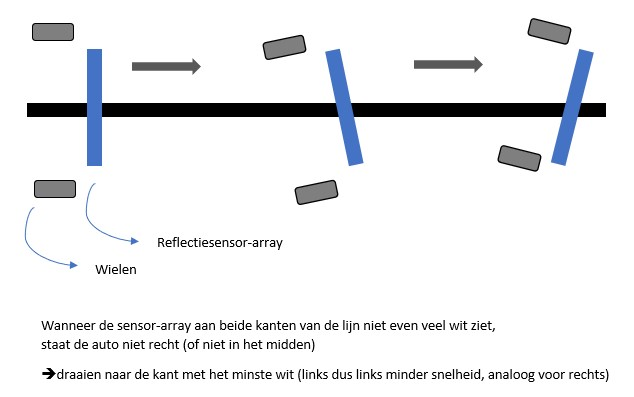
\includegraphics[width=.84\textwidth]{pref2}
	\caption{Het lijnvolgalgoritme laat ons robotwagentje toe om zijn traject te corrigeren indien nodig. Wanneer er links meer wit te zien is, zal het algoritme de wagen naar rechts laten draaien zodat hij de lijn correct volgt. Dit door de linkse motor sneller te laten  }
	\label{fig: lijnvolg}
	
\end{figure}
\subsection{Licht herkennen}
Dit algoritme treedt pas in werking als men een stopstreep detecteert. Dit is zo wanneer de acht sensoren van de reflectiesensor zwart detecteren (zoals in vorige paragraaf beschreven). Met behulp van een while-loop gaan we kijken of het licht groen is dat de kleurensensor detecteert. We gaan gebruik maken van een polling rate van 1 seconde zodat we de myRIO niet overbelasten. Zolang het rood is blijft de while-loop lopen, vanaf de kleurensensor groen ziet, stopt die while-loop en kan het traject verdergezet worden.

\subsection{Andere wagen herkennen en versnellen/vertragen}

Met de afstandssensor kunnen we de afstand tot een voorliggende wagen detecteren. Wanneer de afstand te klein is, gaat de wagen vertragen. Als echter bij het vertragen de kritieke minimale snelheid overschreden wordt (dus nog minder dan de minimale), dan stopt onze wagen (dit is wanneer een andere wagen voor ons stilstaat). Wanneer de snelheid boven een bepaalde waarde is, neemt hij de 'ideale snelheid' aan.

\subsection{Draaien op kruispunt}
We maken een ondersheid tussen drie gevallen; linksaf, rechtsaf en rechtdoor. Bij linksaf moeten we eerst 375mm rechtdoor rijden, dan 90graden naar links draaien om de as van de wagen en tenslotte meer dan 375 mm rechtdoorrijden om dan weer de lijn te volgen.

Bij rechtsaf moet men eerst 125mm rechtdoorrijden, dan 90graden naar rechts draaien om de as van de wagen en tenslotte meer dan 125mm rechtdoorrijden om dan weer de lijn te volgen. Bij rechtdoor moet men meer dan 500mm rechtdoorrijden om dan vervolgens de lijn te volgen. bij deze drie gevallen moet men tijdens het uitvoeren ervan rekening houden of er al dan niet een voorligger zich binnen de zeer kritische gevarenzone bevindt (dit wil zeggen dat de ander wagen voor de een of andere reden stilstaan op het kruispunt)

\subsection{Handmatige Besturing}
Om de controle manueel over te nemen sturen we de motoren rechtstreeks aan. Dit stellen we voor met behulp van twee sliders in LabVIEW. Later zullen we aan die sliders concreet een invulling voor geven om op de test te gebruiken.

\subsection{Implementatie traject}

Vanaf het moment dat we ons traject kennen, kunnen we aan de hand van de vorige algoritmes ons parcours samenstellen. De flowchart van ons programma is terug te vinden in bijlage \ref{sec: flowchart}.

\subsection{Concrete implementatie}
\bigskip
Het hele LabVIEW-programma, gebruikmakend van de voorgenoemde functies splitsen we op in twee stappen:

De eerste stap is wat de auto moet doen tijdens het rijden. Hier moet de auto tegelijk de lijn op de grond volgen, 
een goede afstand tot zijn voorligger behouden (wat dus inhoudt dat die de voorligger moet detecteren en aan de hand van de afstand tot die voorligger zijn snelheid moet aanpassen) 
en de auto moet ook nog eens comfortabel kunnen stoppen,en dus niet te snel rijden, wanneer die een stopstreep detecteert. 
De input voor de snelheid komt van de motoren, de input voor de afstand tot de voorligger komt van de afstandssensor, de lijn en stopstreep detecteren we met de reflectiesensorarray en tot slot het verkeerslicht (dat besproken zal worden in de volgende stap) detecteren we met de kelurensensor.

De tweede stap begint bij de stopstreep van bij het eindd van stap één. 
Wanneer de auto gestopt is aan de stopstreep moet die een verkeerslicht detecteren en daar gepast opreageren, nadat het groen licht geworden is moet die dus over het kruispuntdraaien. 
Daarna moet die een bocht nemen of rechtdoor rijden aan de hand van een vooraf opgesteld parcours. 
Na deze stappen is het algoritme klaar en begint hij weer met stap één.
	
	\subsection{Implementatie traject}
	
	Vanaf het moment dat we ons traject kennen, kunnen we aan de hand van de vorige algoritmes ons parcours samenstellen. De flowchart van ons programma is terug te vinden in bijlage \ref{sec: flowchart}.
	



	\chapter{Bijlagen}
	\section{Planning}
	\label{sec: planning}
	
	\providetranslation[to=Dutch]{Figure}{Figuur}
	
	
	
	\setlist[itemize]{noitemsep, topsep=0pt, leftmargin=*}
	\uselanguage{Dutch}

	\providetranslation[to=Dutch]{Figure}{Figuur}
	
	
	
	\section{Overzicht ontwerpspecificaties}
	\label{sec: ontws}

	
	\bigskip
	
	\begin{figure}
		\centering
		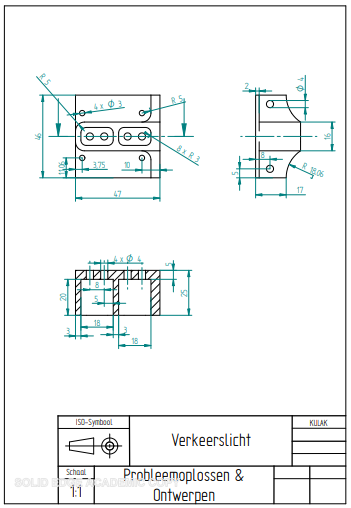
\includegraphics[width=.8\textwidth]{verkeerslicht}
		\caption{Technische tekening verkeerslicht, opgehaald van \cite{artikel1}. }
		\label{fig: verkeerslicht}
	\end{figure}
	\bigskip
	\begin{figure}
		\centering
		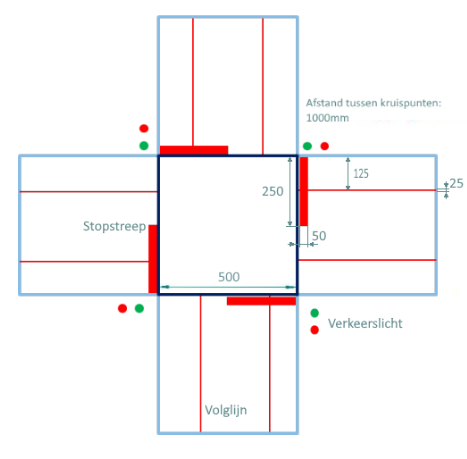
\includegraphics[width=.8\textwidth]{bovenaanzichtkruispunt}
		\caption{Bovenaanzicht kruispunt met relevante maten en items, aangepast vanuit \cite{Smart}.
		}
		\label{fig: kruispunt}
		
	\end{figure}

	

	\bigskip
	
	\section{Teamverantwoordelijkheden}
	\label{seq: vera}
	\includepdf[pages=6]{Team4_planning.pdf}
	
	\section{Takenstructuur}
	\label{sec: taken}
	
			
		\begin{table}
			\centering
			%\caption{Takenstructuur}
			
			Tabel 1: Takenstructuur
			
			% \vspace{\baselineskip}
			\begin{tabular}{p{1cm}p{12cm}c}
				
				
				\toprule
				Code & Taak & Status \\ 
				
				\midrule
				\row{1}{Inwerken}{1}
				\row{2}{Documenten op Toledo lezen}{1}
				
				\row{2}{Ontwerpen en plannen}{1}
				\row{3}{Materiaallijst maken}{1}
				\row{3}{Teamkalender maken}{1}
				\row{3}{Klantenvereisten opstellen}{1}
				\row{3}{Overzicht ontwerpspecificaties}{1}
				\row{3}{Takenstructuur}{1}
				\row{3}{Gantt-grafiek}{1}
				
				\midrule
				\row{1}{Ontwerpen met behulp van de computer}{0}
				\row{2}{3D modellen	(Solid parts)}{1}
				\row{3}{Wiel}{1}
				\row{3}{Motor}{1}
				\row{3}{Motorbeugel}{1}
				\row{3}{Chassis}{1}
				\row{3}{Ballcaster}{1}
				\row{3}{Printplaat}{1}
				\row{3}{Kleursensor}{1}
				\row{3}{Afstandssensor}{1}
				\row{2}{Assemblage (Assembly)}{1}
				
				
				\row{2}{Technische tekeningen (Drawing)}{0}
				
				\row{2}{Stuklijst}{0}
				
				\midrule
				\row{1}{Software}{0}
				\row{2}{Sturen/snelheid regelen}{1}
				\row{2}{Lijnvolgalgoritme}{1}
				\row{2}{Verkeerslichtinterpretatie}{1}
				\row{2}{Voorliggerdetectie}{1}
				\row{2}{Stoppen}{1}
				\row{2}{Vertragen}{1}
				\row{2}{Handmatig besturen}{1}
				\row{2}{Inputs vormgeven}{0}
				\row{2}{Outputs vormgeven}{0}
				\row{2}{Testen}{0}
				
				
				\midrule		
				\row{1}{Rapportering}{0}
				\row{2}{Tussentijds verslag}{1}		
				\row{3}{Nalezen}{1}
				\row{2}{Tussentijdse presentatie}{0}
				\row{3}{Structuur}{1}
				\row{3}{Presentatie maken}{0}
				\row{3}{Nalezen}{0}
				\row{3}{Inoefenen}{0}
				\row{2}{Eindverslag}{0}
				\row{3}{Structuur}{0}			
				\row{3}{Nalezen}{0}
				\row{2}{Eindpresentatie}{0}
				\row{3}{Structuur}{0}
				\row{3}{Presentatie maken}{0}
				\row{3}{Nalezen}{0}
				\row{3}{Inoefenen}{0}
				\bottomrule
			\end{tabular}
		\caption{Takenstructuur}
		\label{tab: taken}
		\end{table}
	\newpage
	
	
	\section{Gantt-grafiek \& Teamkalender}
	\label{sec: kale}
	\includepdf[pages = 7]{Team4_planning}
	\includepdf[pages = 8]{Team4_planning}
	\includepdf[pages = 9]{Team4_planning}
	\includepdf[pages = 10]{Team4_planning}
	\includepdf[pages = 11]{Team4_planning}
	\includepdf[pages = 12]{Team4_planning}
	\includepdf[pages = 13]{Team4_planning}
	
	
	
	\section{Visualisatie ontwerp}
	\label{sec: vis}
	
\begin{figure}[h]
		\centering
		\includegraphics[width=1.2\textwidth]{KS®wagen1.3}
	\caption{CAD-ontwerp van de wagen, samengesteld uit \textit{.par-onderdelen}, gezien vanuit de rechterbovenhoek.}
		\label{fig: wagen}
\end{figure}

\begin{figure}[h]
	\centering
	\includegraphics[width=1.2\textwidth]{KS®skelet.4}
	\caption{Het 3D-geprinte onderdeel \textit{Skelet van de wagen} }.
	\label{fig: skelet}
\end{figure}
%%KS®wagen1.3

\section{Elektrisch circuit}
\label{sec: circ}

\section{Flowcharts}
\label{sec: flowchart}

\begin{figure}
	\centering
	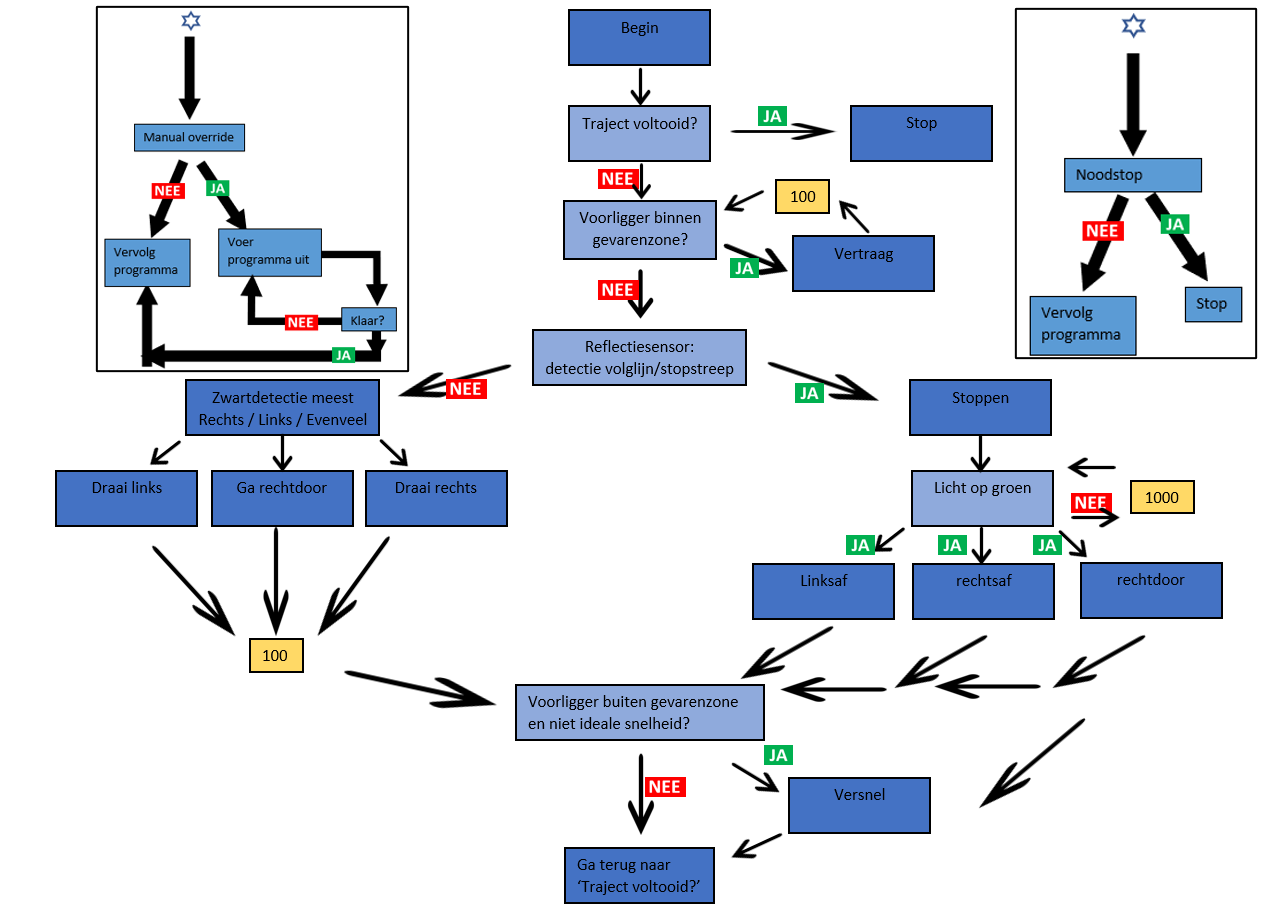
\includegraphics[width=1.3\textwidth]{fchart}
	\caption{De flowchart van ons algoritme. 
	}
	\label{fig: fchart}
	
\end{figure}

\newpage
	\section{Financieel Rapport}
	\label{sec: finrap}
	\subsection*{Hardware}
	
	\begin{table}[h]
		
	
	\begin{tabular}{l|r|r|r}
		Onderdeel& prijs per stuk & aantal & totale prijs \\
		\hline
		Micro Metal Gear Motor 100:1 HP&160 & 2 & 320 \\ 
		
		Dual Drive DRV8833 & 70 & 1 & 70 \\
		Optische afstandsensor (analoog) & 160 & 1 & 160 \\
		TCS34725 Kleur sensor BOB & 150 & 1 & 150 \\
		QTR-8A analoge reflectie sensor array & 150 & 1 & 150 \\
		Oplaadbare LITHIUM-ION & 90 & 2 & 180 \\
		NI MyRio  & 240 & 1 & 240 \\
		Breadboard Tiny & 40 & 1 & 40 \\
		Printplaat & 50 & 1 & 50 \\
		Totaal: 1360
	\end{tabular}
\caption{uitgaven hardware}
\label{tab: ess}
\end{table}
	
	
	\subsection*{Ontwerp}
\begin{table}[h]	
	\begin{tabular}{l|r|r|r}
		
		Onderdeel& prijs per stuk & aantal & totale prijs \\
		\hline
		Ball Caster &60 & 1 & 60 \\
		Wiel 60x8mm zwart &35 & 2 & 70 \\
		Robot Chassis Rechthoekig Zwart &70 & 1 & 70 \\
		
	\end{tabular}
	

	Totaal: 200
	
\caption{uitgaven ontwerp}
\label{tab: ontw}
\end{table}
	
	
	\subsection*{Assemblage}
\begin{table}[h]	
	\begin{tabular}{l|r|r|r}
		Onderdeel& prijs per stuk & aantal & totale prijs \\
		\hline
		Micro metal gear motor beugel &2 & 25 & 50 \\
		Skelet van de wagen &N.A & 1 & N.A\\
		Reflectie sensor houder &N.A & 1 & N.A\\
		
	\end{tabular}
	
	Totaal: 50
	
\caption{uitgaven assemblage}
\label{tab: ass}
\end{table}
	\subsection*{Onkosten}

\begin{table}[h]

	\begin{tabular}{l|r}
		kost& waarde \\
		\hline
		Bieding &1300 \\
		
		
	\end{tabular}
	\newline
	Totaal: 1300
\caption{uitgaven onkosten}
\label{tab: onk}
\end{table}
	
	\subsection*{Niet gebruikt}
	Totaal: 590
	
\begin{figure}[h]
	\centering
	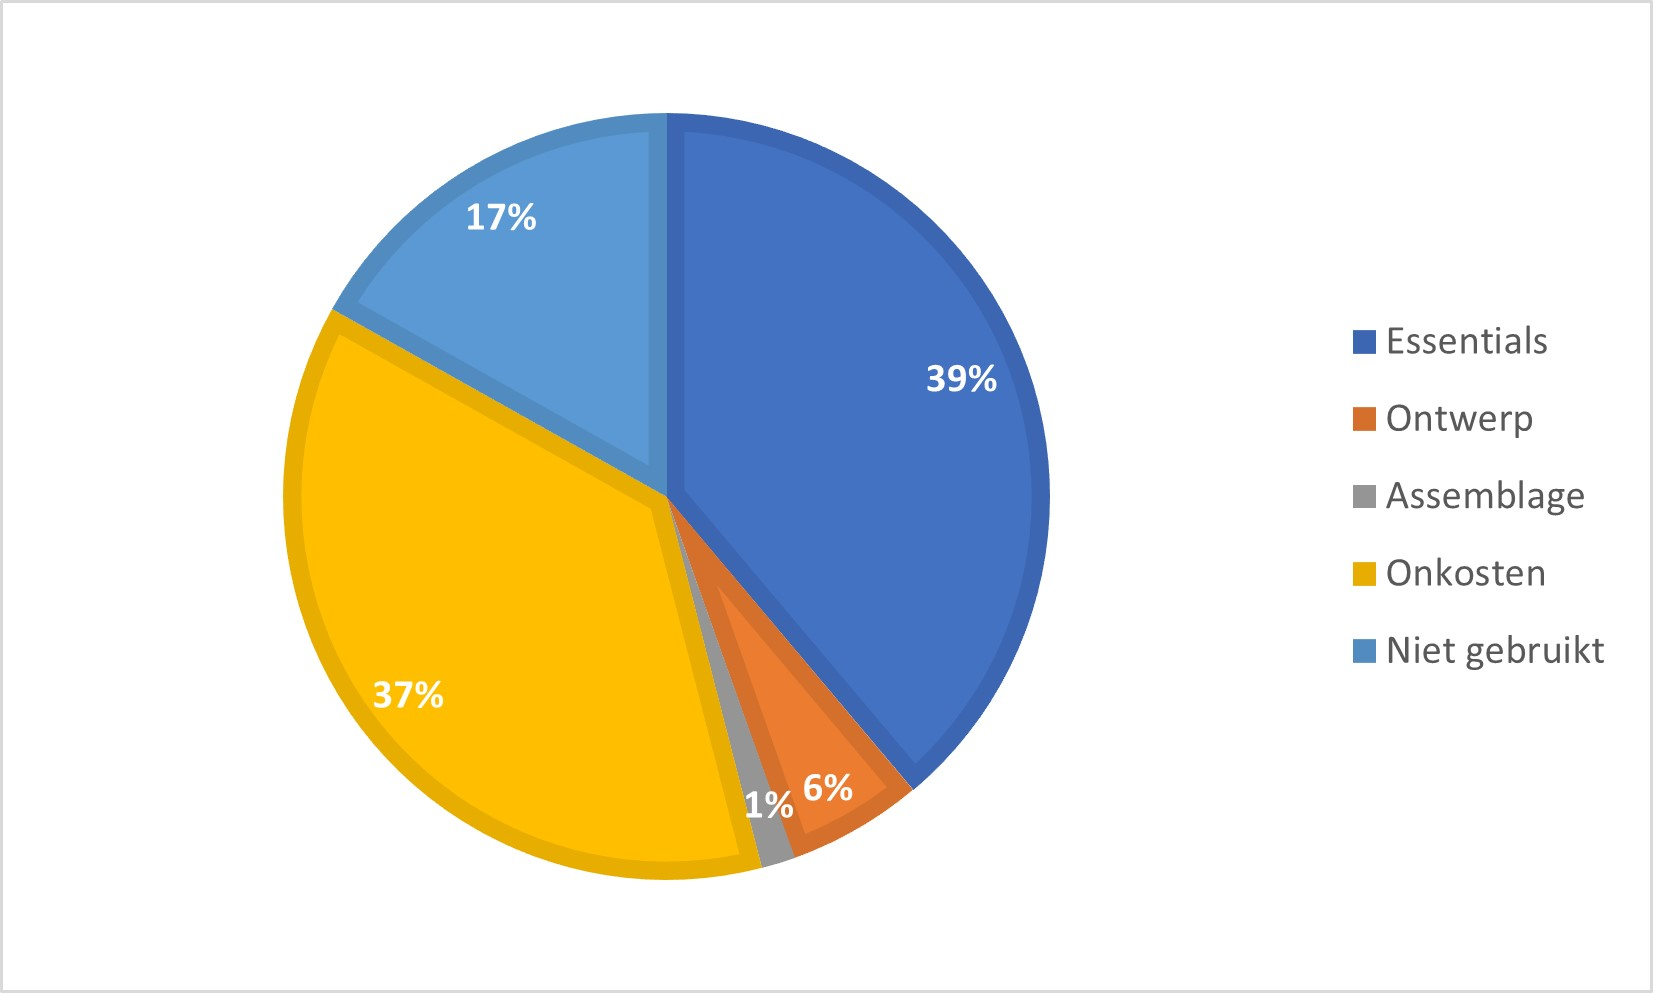
\includegraphics[width=1.2\textwidth]{pie}
	\caption{Visualisatie van de besteding van ons budget }
	\label{fig: pie}
\end{figure}
	
	
	
	
	
	
	
	%%referenties
	\bibliography{bibliografie_verslag.bib}
	\bibliographystyle{unsrt}
	
	
	
	%%Bijlagen
	
\end{document}